\chapter{Sistemas de refrigeración}

\section{Compresores}

\subsection{Clasificación según su construcción}
\begin{itemize}
    \item \textbf{Compresores abiertos:} Muy usados en la industria. Permiten mantenimiento y reparación. Se usan con amoníaco ya que este gas corroe el cobre, por lo tanto, no se pueden usar compresores herméticos.
    
    \item \textbf{Compresores herméticos o cerrados:} Usados principalmente en sistemas comerciales y residenciales. El motor está sellado junto al compresor, lo que limita el mantenimiento.
    
    \item \textbf{Compresores semiherméticos:} Permiten cierto mantenimiento sin estar completamente abiertos.
\end{itemize}

\subsection{Tipos de compresores}

\subsection{Características y selección}

\subsubsection{Relación de compresión} Es la relación entre la presión de succión y la de descarga.

\subsubsection{Capacidad de un compresor}

\parencite{Pág. 200 R11-2.1}{ari1}


Cuando los compresores tienen menos carga, funcionan a una presión de succión inferior, reduciéndose su capacidad. Cuando se incrementa la carga, se eleva la presión de succión, incrementando la capacidad del compresor. Conforme se reduce la temperatura del evaporador, se incrementa el volumen específico, se reduce la densidad del refrigerante y se bombean menos libras de refrigerante.


El control de capacidad en un compresor se puede efectuar i) cambiando el refrigerante (no recomendado) y ii) por cambios en el desplazamiento de dicho compresor. Existen 6 formas de realizar cambios en el desplazamiento:
\begin{enumerate}
    \item On-Off
    \item On-Off de varias máquinas
    \item Descarga de cilindros. Creo que deshabilita cilindros para que no desplace tanto volumen.
    \item Derivación de gases calientes. Se aplica solo para variaciones pequeñas. Aumento de sobrecalentamiento en el compresor. No es eficiente en el uso de energía. \emph{Lo más comúnmente utilizado en compresores a tornillo para el control de capacidad por derivación de gases son válvulas correderas a la entrada del compresor}.
    \item Variador de velocidad
    \item Aletas de entradas moduladoras (compresores centrífugos)
\end{enumerate}

\subsection{Lubricación}
\parencite{Pág. 201 R11-3}{ari1}



Todos los compresores de refrigeración requieren lubricar sus superficies en movimiento. La distribución del lubricante puede ser mediante 1) sistemas de salpicado o 2) sistemas de alimentación a presión, por bomba de aceite independiente. Como se espera que parte del lubricante sea transportada junto con el gas de descarga, el aceite debe ser miscible con el refrigerante y compatible con el sistema diseñado.


Los lubricantes que se utilizan en sistemas herméticos y semiherméticos tienen que ser compatibles con los componentes eléctricos y ser buenos aislantes.



\subsection{Protecciones del compresor}
\begin{itemize}
\item \textbf{Eléctricas:} Termomagnética, protector térmico.
\item \textbf{Mecánicas:} Termostatos, controles de presión en succión y descarga, sensor de temperatura en el cárter para proteger el aceite.
\end{itemize}

\subsection{Control y seguridad}
\subsubsection{Controles del compresor}
\begin{itemize}
\item Presión de succión y descarga
\item Temperatura del aceite
\item Temperatura de descarga
\item Corriente del motor
\end{itemize}

\subsubsection{Información para protecciones}
\begin{itemize}
\item Se usan presostatos (succión y descarga) y termostatos (descarga, cárter). Están ubicados estratégicamente para evitar sobrepresiones, sobrecalentamiento y problemas de lubricación.
\end{itemize}

\subsection{Dimensionamiento y selección de compresor}
 Se requiere conocer:
\begin{itemize}
    \item \textbf{Capacidad frigorífica}: Obtenido del estudio de cargas + un 8\% por el sobrecalentamiento en tuberías (fuente: creeme o buscalo por ahí).
    \item \textbf{Tipo de refrigerante}: Cambia las características en el sistema, se puede ver fácilmente con el diagrama de Mollier Ph.
    \item \textbf{Condiciones de evaporación y condensación}: Temperaturas y presiones.
    \item \textbf{Caudal másico}: Calculado en función del calor a extraer y la diferencia de entalpías en el evaporador.
    \item \textbf{Requerimientos eléctricos}: Frecuencia y tensión.
\end{itemize}

\subsection{Comparación entre compresores a tornillo y alternativos}
\begin{itemize}
\item \textbf{Compresor a tornillo:} Mayor eficiencia, capacidad de regulación continua, menos vibraciones.
\item \textbf{Compresor alternativo:} Tiene volumen muerto, menos eficiente, útil en sistemas pequeños.
\end{itemize}

\subsection{Volumen aspirado en la succión}
Es fundamental porque afecta directamente la capacidad del compresor. Un mayor volumen aspirado significa mayor capacidad frigorífica.

\subsection{Migración de refrigerante y arranque inundado}

La \emph{migración de refrigerante} ocurre cuando el refrigerante en forma de vapor se desplaza hacia el cárter del compresor durante los periodos en los que el equipo está detenido. Una vez en el cárter, el refrigerante condensa debido a la baja temperatura y se acumula en el fondo, generando dos zonas: una de refrigerante líquido y otra de aceite. El refrigerante se separa  del aceite y, debido a su mayor densidad, se deposita en el fondo del cárter.

El \emph{arranque inundado} es una consecuencia de esta migración y se produce al poner en marcha el compresor. Debido a la diferencia de presiones de vapor entre el refrigerante y el aceite, la caída brusca de presión provoca una evaporación rápida del refrigerante en el aceite. Esto genera una espuma dentro del cárter que desplaza el lubricante, impidiendo la correcta lubricación del compresor y generando un riesgo de daño mecánico. (¿Se podría decir que se produce flash gas? Algo similar a lo que sucede en la válvula de expansión.)

\begin{figure}[h]
    \centering
    \begin{subfigure}{.3\linewidth}
    \centering
    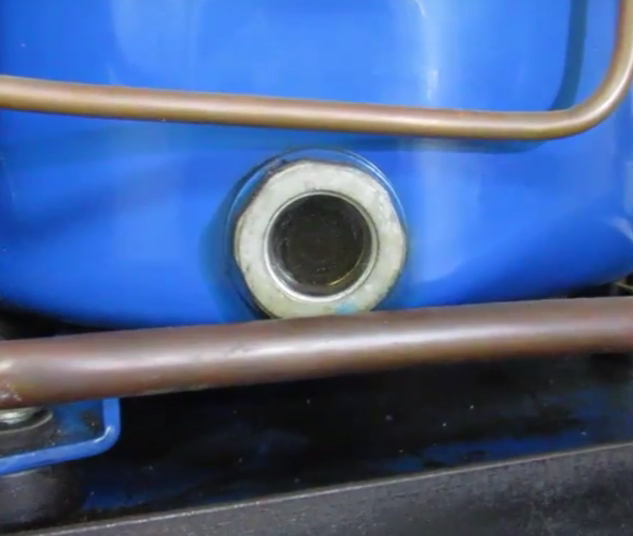
\includegraphics[height=4cm]{vapor/arranque-1}
    \caption{Antes del arranque}
    \end{subfigure}
    \begin{subfigure}{.3\linewidth}
    \centering
    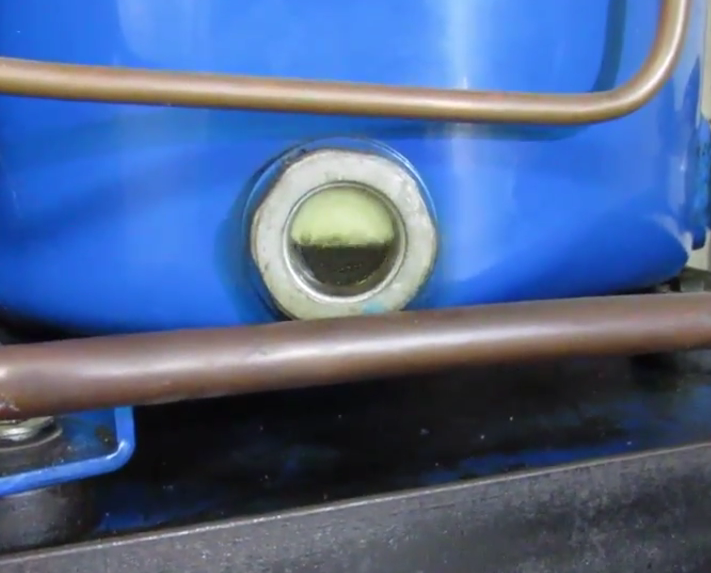
\includegraphics[height=4cm]{vapor/arranque-2}
    \caption{Inmediatamente en el arranque}
    \end{subfigure}
    \begin{subfigure}{.3\linewidth}
    \centering
    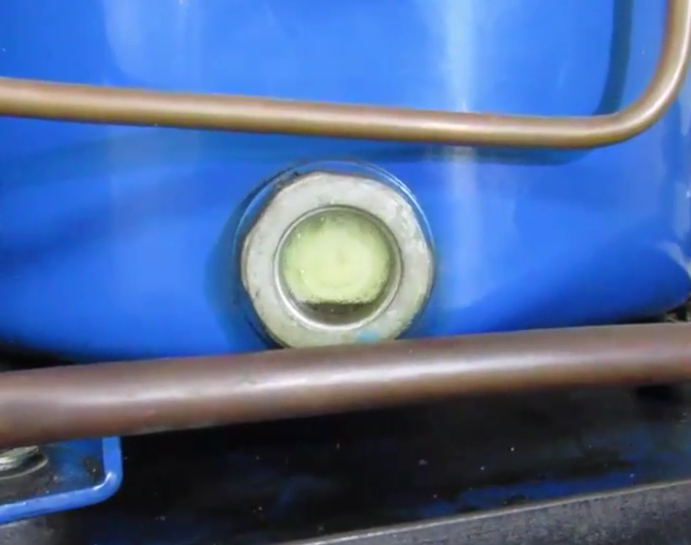
\includegraphics[height=4cm]{vapor/arranque-3}
    \caption{Posterior al arranque}
    \end{subfigure}
    \caption{Mirilla de un compresor durante un arranque inundado.}
    % \label{fig}
\end{figure}

Medidas preventivas:
\begin{itemize}
    \item Instalar resistencias de cárter, que mantienen el refrigerante en estado gaseoso antes del arranque.
    \item Evitar ubicar el compresor en lugares con temperaturas ambientales muy bajas, ya que disminuyen la presión de vapor del refrigerante.
    \item No sobrecargar el sistema con refrigerante, respetando la capacidad máxima especificada para el compresor o unidad condensadora.
    \item Implementar un sistema de apagado por pump-down, que consiste en cortar la alimentación de refrigerante, permitiendo que el compresor comprima y recupere el refrigerante de la línea de succión, almacenándolo posteriormente en el acumulador de líquido.
\end{itemize}

\section{Válvulas}


\subsection{Tipos de válvulas}
\begin{itemize}
\item \textbf{Para regular caudal:} Válvula de expansión termostática o electrónica.
\item \textbf{Para bloquear:} Válvula de bola, válvula de cierre.
\end{itemize}

\subsubsection{Válvulas de expansión termostática}
Utilizadas como control del flujo del refrigerante.
Dentro de las válvulas de expansión termostática (VET) se tienen:
\begin{itemize}
    \item \textbf{VET con compensación interna (común):} encargada de reducir la presión del refrigerante. Regula el caudal en función del recalentamiento, considerando la \emph{presión a la entrada del evaporador}. La aguja se equilibra considerando la presión ejercida por el bulbo —que refleja la temperatura del bulbo—, el ajuste del resorte y la presión en la entrada del evaporador. Este tipo de válvula debe instalarse cuando la caída de presión dentro del evaporador es despreciable o muy pequeña.

    Pero si dentro del evaporador hay una caída de presión (por ejemplo, si es largo, sucio o mal diseñado), no refleja bien lo que pasa al final del evaporador.
    
    \item \textbf{VET con compensación externa:} se utiliza cuando existe una caída de presión significativa en el evaporador. La aguja se equilibra en función del ajuste del resorte, la presión ejercida por el bulbo y la \emph{presión al final del evaporador}. Esta solución es adecuada para evaporadores grandes o con pérdidas de presión considerables, ya que la válvula con compensación interna no puede detectar ni compensar estas caídas de presión. 
\end{itemize}

\begin{figure}[h]
  \centering
  \begin{subfigure}{.4\linewidth}
      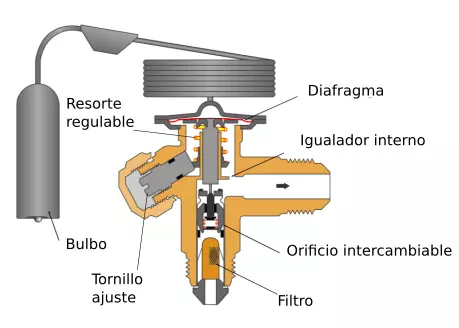
\includegraphics[width=\linewidth]{vapor/valv-1}
      \caption{Esquema de una VET}
  \end{subfigure}
  \begin{subfigure}{.25\linewidth}
      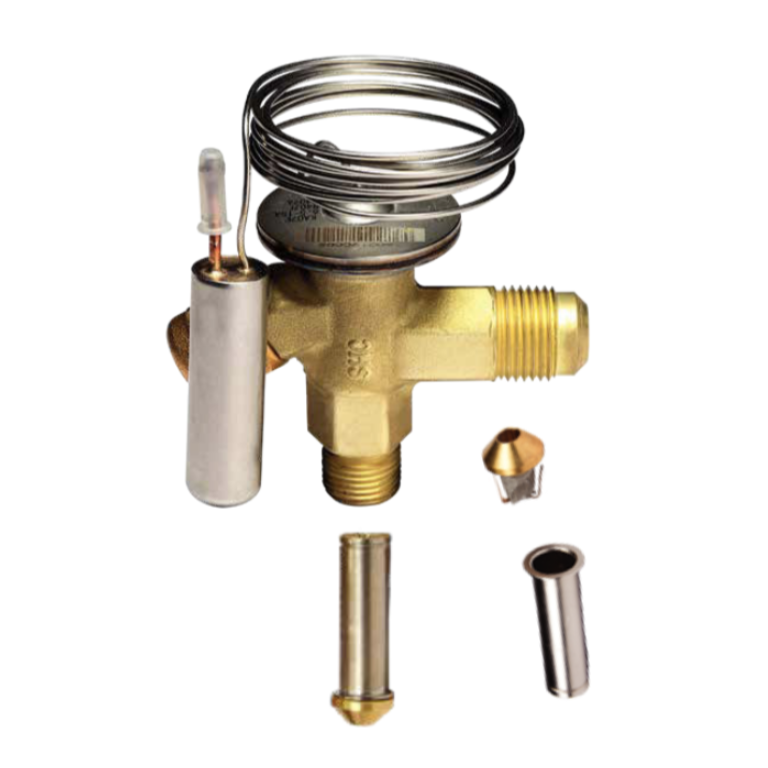
\includegraphics[width=\linewidth]{vapor/valv-2}
      \caption{VET sin compensación}
  \end{subfigure}
  \begin{subfigure}{.25\linewidth}
      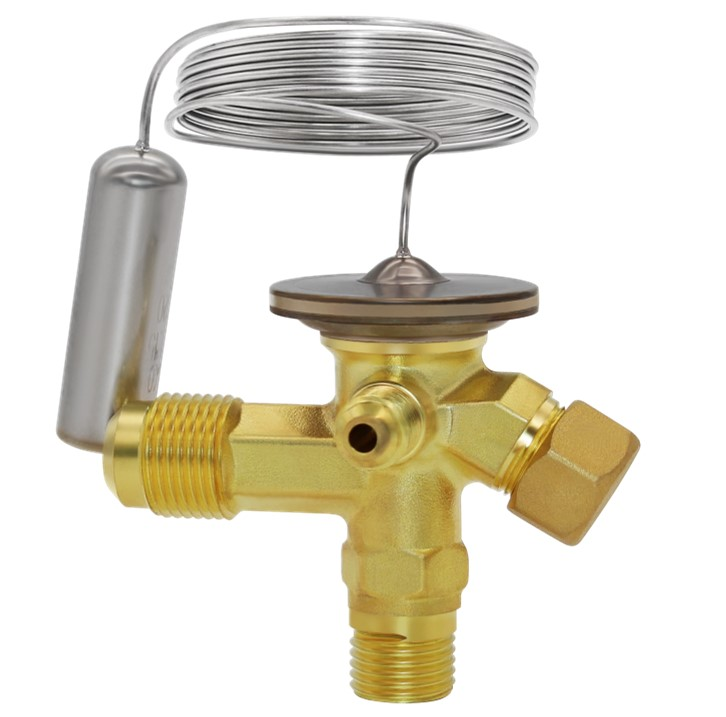
\includegraphics[width=\linewidth]{vapor/valv-3}
      \caption{VET con compensación}
  \end{subfigure}
  \caption{Válvulas de Expansión Termostática (VET).}
   \label{fig:tres_imagenes}
\end{figure}

\subsubsection{Válvulas de servicio o rotalock}
Son utilizadas para cerrar los circuitos, aislar zonas para mantenimiento y para puntos de medición por las tomas de servicio.

Tienen tres posiciones principales, según cómo esté el bástago dentro de la válvula:
\begin{enumerate}
    \item Abierto en banda: hay conexión entre la tubería y el recipiente donde está instalada (compresor, acumulador, separador, etc). El puerto de servicio está cerrado.
    \item Posición intermedia: hay conexión entre la tubería y el recipiente donde está instalada. El puerto de servicio está abierto para que se puedan conectar instrumentos de medición.
    \item Cerrado en banda: la tubería ya no está conectada con el recipiente, el puerto de servicio está abierto y las lecturas van a estar sobre el recipiente.
\end{enumerate}

Existen aquellas que tienen dos tomas de servicio pero solo una de ellas se podrá cerrar, la otra permanecerá siempre abierta. La toma que siempre está en conexión con el circuito se utiliza para conectar elementos de protección, como presostatos de seguridad, con la finalidad de que nadie pueda retirarlos y siempre estén conectados si el sistema está en funcionamiento. Aunque, como precaución tienen válvulas con obús para impedir el escape de gas.

\begin{figure}[h]
  \centering
  \begin{subfigure}{.3\linewidth}
      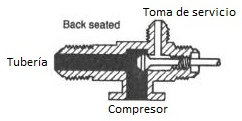
\includegraphics[width=\linewidth]{vapor/posvs-1}
      \caption{Abierto en banda}
  \end{subfigure}
  \begin{subfigure}{.3\linewidth}
      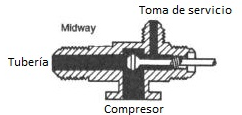
\includegraphics[width=\linewidth]{vapor/posvs-2}
      \caption{Posición intermedia}
  \end{subfigure}
  \begin{subfigure}{.3\linewidth}
      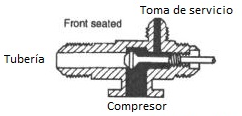
\includegraphics[width=\linewidth]{vapor/posvs-3}
      \caption{Cerrado en banda}
  \end{subfigure}
  \caption{Posiciones de una válvula de servicio conectada al compresor.}
  % \label{fig:tres_imagenes}
\end{figure}

\subsubsection{Válvulas de paso y cierre}

Estos tipos de válvulas tienen el fin de aislar el circuito o servir como bypass.
Pueden ser del tipo globo o de bola, y de diafragma.

\begin{figure}[h]
  \centering
  \begin{subfigure}{.35\linewidth}
      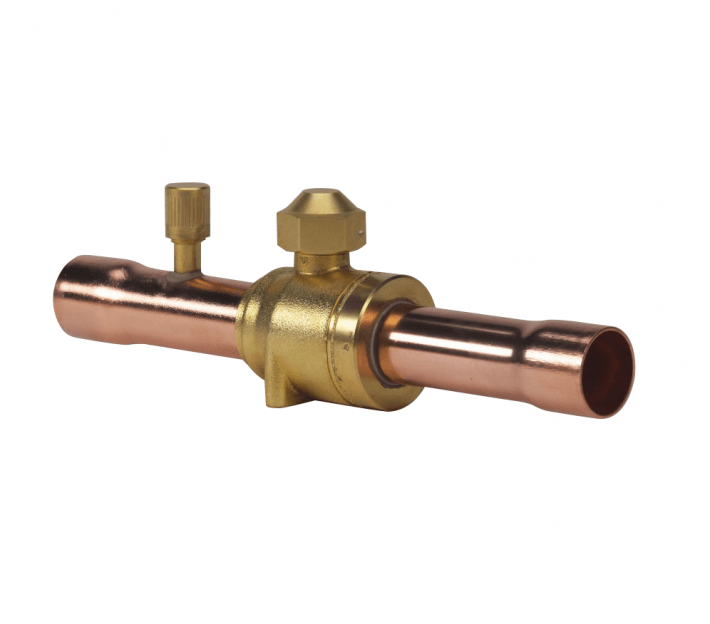
\includegraphics[width=\linewidth]{vapor/globo}
      \caption{Válvula globo}
  \end{subfigure}
  \begin{subfigure}{.25\linewidth}
      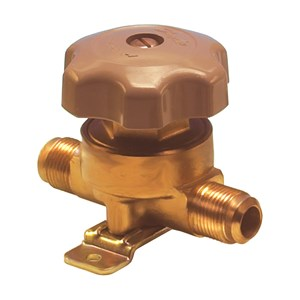
\includegraphics[width=\linewidth]{vapor/diafragma}
      \caption{Válvula de diafragma}
  \end{subfigure}
  \caption{Válvulas de paso y cierre.}
\end{figure}

\subsubsection{Válvulas de retención}

Las válvulas check permiten el flujo en una sola dirección y evitan el retorno del fluido. A continuación, se describen los tipos más comunes:

\begin{itemize}
    \item \textbf{Válvula check de clapeta}: utilizada en líneas de descarga de compresores. Se abre con la presión del refrigerante cuando el compresor está funcionando y se cierra cuando se detiene, evitando que el refrigerante fluya en sentido inverso hacia el compresor.


    \item \textbf{Válvula check de disco}: el disco se levanta verticalmente con el flujo y cae para sellar cuando el flujo se invierte. Requiere instalación en posición horizontal y suele usarse en aplicaciones de alta presión.


    \item \textbf{Válvula check de resorte (spring-loaded check valve):}  tiene un resorte que mantiene cerrada la válvula hasta que la presión del refrigerante es suficiente para abrirla. Se utiliza en líneas de líquido o de gas para controlar el sentido del flujo. Su diseño permite instalarla en distintas posiciones.

\end{itemize}

\begin{figure}[h]
  \centering
  \begin{subfigure}{0.25\linewidth}
    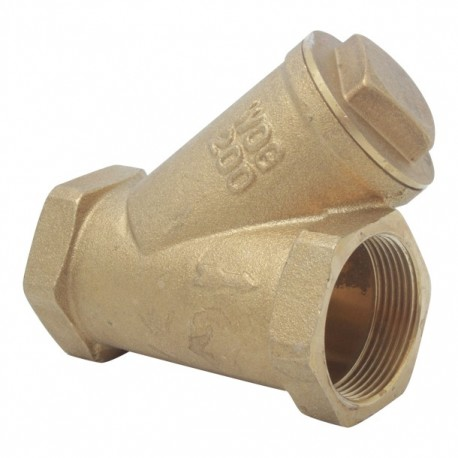
\includegraphics[width=\linewidth]{vapor/check-1}
  \end{subfigure}
  \begin{subfigure}{0.25\linewidth}
    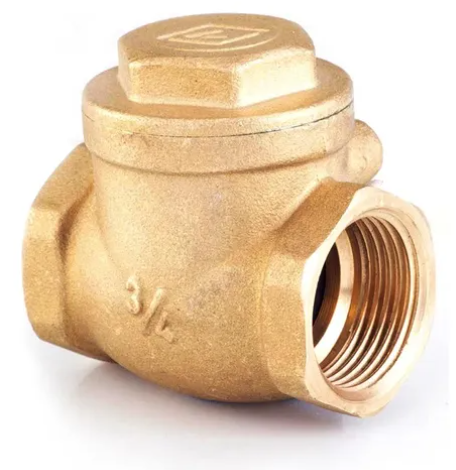
\includegraphics[width=\linewidth]{vapor/check-2}
  \end{subfigure}
  \begin{subfigure}{0.2\linewidth}
    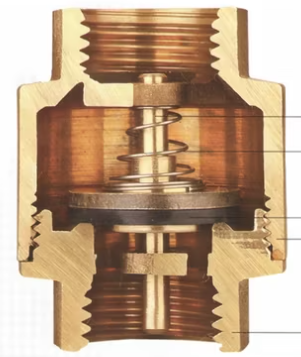
\includegraphics[width=\linewidth]{vapor/check-dentro}
  
  \end{subfigure}
  \caption{Válvulas de retención de tipo disco y resorte.}
  \label{fig:main}
\end{figure}




\section{Evaporadores}
Son encargados de absorber el calor del ambiente mediante el refrigerante frío que circula por su interior. Existen los siguientes tipos
\begin{itemize}
    \item De tubos: conformados por tubos desnudos (serpentines) con refrigerante circulando en su interior. Pueden estar sumergidos o al aire. 
    \item De tubos y placas: son tubos con aletas o placas colocadas en forma transversal. El  objetivo de las aletas es aumentar la superficie de contacto que si solo se tuvieran tubos desnudos, pero el abuso de esto podría ser una limitante del aire que pasa a través del serpentín. Si se trabaja a muy bajas temperaturas, la distancia entre aletas no debe ser tan pequeña por el acumulamiento de escarcha.
    \item De placas: constan de placas unidas herméticamente con un circuito trazado en su interior, ya sea conformado en las mismas placas o por conductos instalados dentro.
\end{itemize}

\subsection{Clasificación}

Se pueden clasificar según la \emph{circulación del aire a través del evaporador}, la \emph{alimentación del refrigerante} y la \emph{transmisión de frío}.

\begin{itemize}
\item La circulación del aire a través del evaporador:\begin{itemize}
    \item De convección natural: el movimiento de aire se da por diferencias en la densidad (el calor sube y el frío baja).
    \item De convección forzada: el movimiento de aire se produce por ventiladores
    \end{itemize}
\item La alimentación del refrigerante:\begin{itemize}
    \item De expansión seca: al evaporador ingresa una mezcla de de líquido y gas refrigerante, salidos de la válvula de expansión. Son más eficientes para pequeñas instalaciones, más económicos y los más usuales.
    \item Inundados: al evaporador ingresa líquido refrigerante, salido de un acumulador o colector de líquido.
    \item Sobrealimentados: es un conjunto de evaporadores inundados con la diferencia de que el líquido refrigerante es impulsado por una bomba de circulación para superar las caídas de presión.
\end{itemize}
\item La transmisión de frío:\begin{itemize}
    \item De expansión directa: el espacio a refrigerar está en contacto directo con el serpentín de refrigerante.
    \item De expansión indirecta: se utiliza un refrigerante secundario que estará en contacto directo en el espacio a refrigerar, generalmente se trata de agua. El refrigerante (primario) enfría el agua (secundario) y luego esta se distribuye a las zonas requeridas.
\end{itemize}
\end{itemize}

\subsection{Selección}

El evaporador se selecciona según el calor a extraer -capacidad de refrigeración- y el salto térmico o diferencial de temperatura Dt. Posterior a eso, se debe verificar la presión del ventilador y el caudal de aire que maneja.

El tipo de producto y las condiciones internas establecen la temperatura a la que trabajará el evaporador. Cada fabricante debería facilitar tablas de humedad relativa vs diferencial de temperatura. La humedad relativa y la temperatura interna son condición de diseño o producto, y a partir de ahí se obtiene la temperatura de evaporación
\[\triangle t = t_i - t_e\]

La capacidad de refrigeración se calcula en función del análisis de cargas térmicas.

\section{Condensadores}

\subsection{Selección y dimensionamiento}
\begin{itemize}
\item De catálogo: Considerar capacidad de rechazo de calor, tipo de refrigerante, condiciones ambientales.
\end{itemize}

\subsection{Condensadores evaporativos}
\begin{itemize}
\item Se seleccionan según capacidad térmica, condiciones de bulbo húmedo, tipo de refrigerante, presión de condensación.
\end{itemize}

\section{Cámara Frigorífica}
Como norma general:
\begin{itemize}
    \item Seguir lineamiento establecidos por senasa, cuando de alimentos se trata
\end{itemize}

\subsection{Tipos de cámaras}
Para carnes, pero me imagino que para cualquier producto, se tienen los siguientes tipos de cámaras
\begin{itemize}
    \item De enfriamiento
    \item De conservación de productos enfriados (1 a 10°C para carnes)
    \item De congelación (-15 a -18 °C para carnes)
    \item De conservación de productos congelados (-18°C para carnes)
\end{itemize}

\subsection{Aislación}

\begin{itemize}
\item Consideraciones: Buen aislamiento térmico, control de humedad, control de temperatura.
\item Materiales: Paneles de poliuretano expandido, acero inoxidable para superficies interiores.
\item Cargas: Producto almacenado, renovación de aire, apertura de puertas.
\item Cortinas de vapor: Minimizar ingreso de aire húmedo.
\item Evaporadores: Ubicación en zona alta, circulación de aire forzada.
\item Caudal de aire: Determinado por el diseño del evaporador, asegura distribución homogénea.
\end{itemize}

\section{Controles}

\subsection{Controles básicos}
Arrancan y detienen los componentes del sistema.
\begin{itemize}
    \item Termostatos
    \item Presostatos
    \item Humidistatos
\end{itemize}

\subsection{Controles de operación}
Regulan los procesos. Tengo entendido que pueden ser activados por los componentes de los controles básicos (además de otros, seguramente).

\begin{itemize}
    \item Relevadores, contactores, arrancadores.
    \item Válvula solenoide (electroválvula): Cuando se energiza el solenoide, el émbolo en su interior se mueve para controlar el flujo de la línea. Se utiliza para el control del fluido refrigerante y se coloca en la línea de líquido después de la válvula de expansión.
    \item Válvula de cuatro vías (inversora): Utilizada para que el sistema actúe como bomba de calor (para calefacción). Tiene 4 conexiones: la central inferior para la descarga del compresor, la central superior para la succión del compresor y las otras dos dependerán si el sistema trabaja para refrigeración o calefacción.
    \item Válvulas de contrapresión (reguladora de presión de succión). Utilizada para mantener una temperatura constante en el evaporador.
    \item Válvulas de una vía (antiretorno): Permite el flujo del refrigerante en una dirección.
\end{itemize}

\subsection{Arranque pump-down}

Se utiliza un termostato para controlar la electroválvula y un presostato para encender o apagar el compresor.

\section{Circuitos y Diagramas}

Los circuitos posibles -pero no los únicos- son:
\begin{itemize}
    \item Básico: incluye compresor, evaporador, condensador, válvula de expansión, separador de aceite, acumulador de succión, acumulador de líquido, válvulas de servicio, cierre y check, presostatos de seguridad, reguladores de presión, manómetros (hasta qué punto se considera básico esto?), válvula solenoide, filtros, mirilla y válvulas de cierre según requerimiento.
    
    \item Con evaporador inundado, incluiría todo lo anterior pero en vez de un acumulador de líquido sería un tanque de líquido. Del tanque de líquido salen dos líneas principales: para el evaporador (todo líquido) y para la succión (todo gas). Seguro faltan más cosas.

    \item Con refrigerante recirculado, con todos los componentes del anterior pero se agrega una bomba para recircular el refrigerante en el evaporador. Viene a solucionar el problema del aceite (estancado no sería la palabra) en el evaporador, ya que la bomba tiene la sufiente presión para empujar el aceite y retorne al tanque de líquido.
    
    \item Con dos evaporadores en la misma cámara o en cámaras separadas. En el primero, por cada evaporador, se tiene una VET. En el segundo se agrega una electroválvula y una VET a cada uno junto con válvulas de cierre ya que el cierre depende de la temperatura en cada sector.
    
    \item Con descongelación por gas caliente: se deriva de la línea de descarga una tubería dirigida al evaporador, debido a que este funcionará como condensador del refrigerante cuando atraviese caliente a través y transfiera su calor a la escarcha en el evaporador. Se instala en esa línea una válvula solenoide y una check.

    \item Con descongelación por inversión: se instalan una VET más y 2 derivaciones con válvulas antiretorno. Cuando hay escarcha en el evaporador, el sentido de flujo de refrigerante cambia y se utiliza al condensador como evaporador y al evaporador como condensador. Con un circuito se va a entender más seguramente.
\end{itemize}

\begin{itemize}
\item Circuito de vapor a dos cargas: Caldera, válvula reductora de presión, derivaciones con trampas de vapor, válvulas de seguridad y control. Considerar pérdidas por distancia.
\item Comportamiento del vapor: Expansión al reducir presión, condensado debe drenar con pendiente y trampas.
\end{itemize}

\section{Recalentamiento y Subenfriamiento}

Estos fenómenos se dan en parte dentro del condensador y del evaporador:
\begin{itemize}
\item Recalentamiento: se da al final del evaporador (recalentamiento útil) y en la línea de succión. Es necesario para asegurar que llegue solo refrigerante en estado gaseoso al compresor y evitar daños. Sin embargo, un exceso de recalentamiento, provocaría que luego de la compresión el refrigerante tenga temperaturas demasiado elevadas pudiendo ser perjudicial.
\item Subenfriamiento: se da al final del condensador y parte de la tubería de líquido. Es necesario para aumentar la capacidad frigorífica y que menor cantidad de refrigerante se transforme en gas durante la expansión.
\end{itemize}
